Le premier type de contraintes sur les poids des réseaux morphologiques est celui porté sur la géométrie des noyaux $w$ des couches de ces réseaux. 
Sont développées et étudiées dans cette sous-partie les différentes métriques de contraintes géométriques utilisées pendant le stage. On distingue ici cinq contraintes géométriques : l'erreur sur le centre de masse $C_\text{center}$ ; l'erreur sur la dispersion $C_\text{disp}$ ; l'erreur sur la symétrie $C_\text{sym}$ ; l'erreur sur la binarité $C_\text{binary}$ ; et l'erreur sur la norme $C_\text{norm}$. \\
%$\mathcal{S}$MorphNetTanh
\vspace{0.0mm}


%%%%%%%%%%%%%%%%%%%%%%%%%%%%%%%%%%%%%%%%%%%%%%%%%%%%%%%%%%%%%%%%%%%%%%%%%%%%%%%%%%%%%%%%%%%%%%%%%%%%%%%%%%%%%%
%%%%%%%%%%%%%%%%%%%%%%%%%%%%%%%%%%%%%%%%%%%%% 1e contrainte %%%%%%%%%%%%%%%%%%%%%%%%%%%%%%%%%%%%%%%%%%%%%%%%%%
%%%%%%%%%%%%%%%%%%%%%%%%%%%%%%%%%%%%%%%%%%%%%%%%%%%%%%%%%%%%%%%%%%%%%%%%%%%%%%%%%%%%%%%%%%%%%%%%%%%%%%%%%%%%%%

\noindent \textbf{a. Erreur sur le centre de masse}\\
\vspace{-0.6mm}

La première métrique de contrainte géométrique sur les noyaux $w$ des réseaux morphologiques est l'erreur sur le centre de masse, notée $C_\text{center}$. Soit $w: W \subseteq \mathbb{Z}^2 \rightarrow \mathbb{R}$ un noyau de couche. On prolonge $\mathbb{Z}^2$ dans $\mathbb{R}^2$, et on considère $\mathbb{R}^2$ comme un espace vectoriel muni de la norme euclidienne $\| \text{\raisebox{\mylen}{\tiny$\bullet$}} \|$. Le centre de masse $p_w \in \mathbb{R}^2$ de $w$ est défini par :

\vspace{-3.4mm}
\begin{equation}
    p_w = \frac{1}{\sum_{x \in W} w(x)} \sum_{x \in W} w(x) x
    \label{mass_center}
\end{equation}


\newpage

\vspace{3.6mm}
Soit $p_c \in \mathbb{R}^2$ le point << central >> visé, et soit $\zeta > 0$ (par défaut, $\zeta = 2$). L'erreur $C_\text{center}$ sur le centre de masse $p_w$ de $w$ par rapport à $p_c$ est définie par :

\vspace{2.6mm}
\begin{equation}
    C_\text{center}(w, p_c)_\zeta = \frac{ \left \| p_w - p_c \right \| ^\zeta }{ \sup_{p \in W} \left \| p - p_c \right \| ^\zeta }
    \label{erreur_center}
\end{equation}

\vspace{6.4mm}
Dans la pratique, on voudra faire tendre le centre de masse $p_w$ du noyau $w$ vers le centre de son support $W$ (de taille finie) dans $\mathbb{R}^2$. Dans ce cas : $p_c = \frac{1}{|W|} \sum_{x \in W} x$ . \\

%\vspace{-1.8mm}
\noindent Prenons par exemple l'expérience avec \textit{disk3} pour la fermeture sur FashionMNIST. La figure ci-après montre l'évolution de la convergence des deux noyaux du réseau, avec des checkpoints à différents stades durant l'entraînement, sans et avec cette contrainte $C_\text{center}$ dans la \textit{loss} (avec $\lambda = 0.01$). Dans les deux cas, le réseau possède le partage de poids doux tel que décrit précédemment. On obtient les mêmes résultats sur 6 runs. \\

%%% A chaque fois, faire deux comparaisons (schéma de l'évolution du filtre sur plusieurs périodes) : l'une sans la contrainte (prendre un truc qui converge mal), l'autre avec (prendre un truc qui converge bien) !

%figure
\vspace{0.6mm}
\begin{figure}[htp]
  \begin{center}
    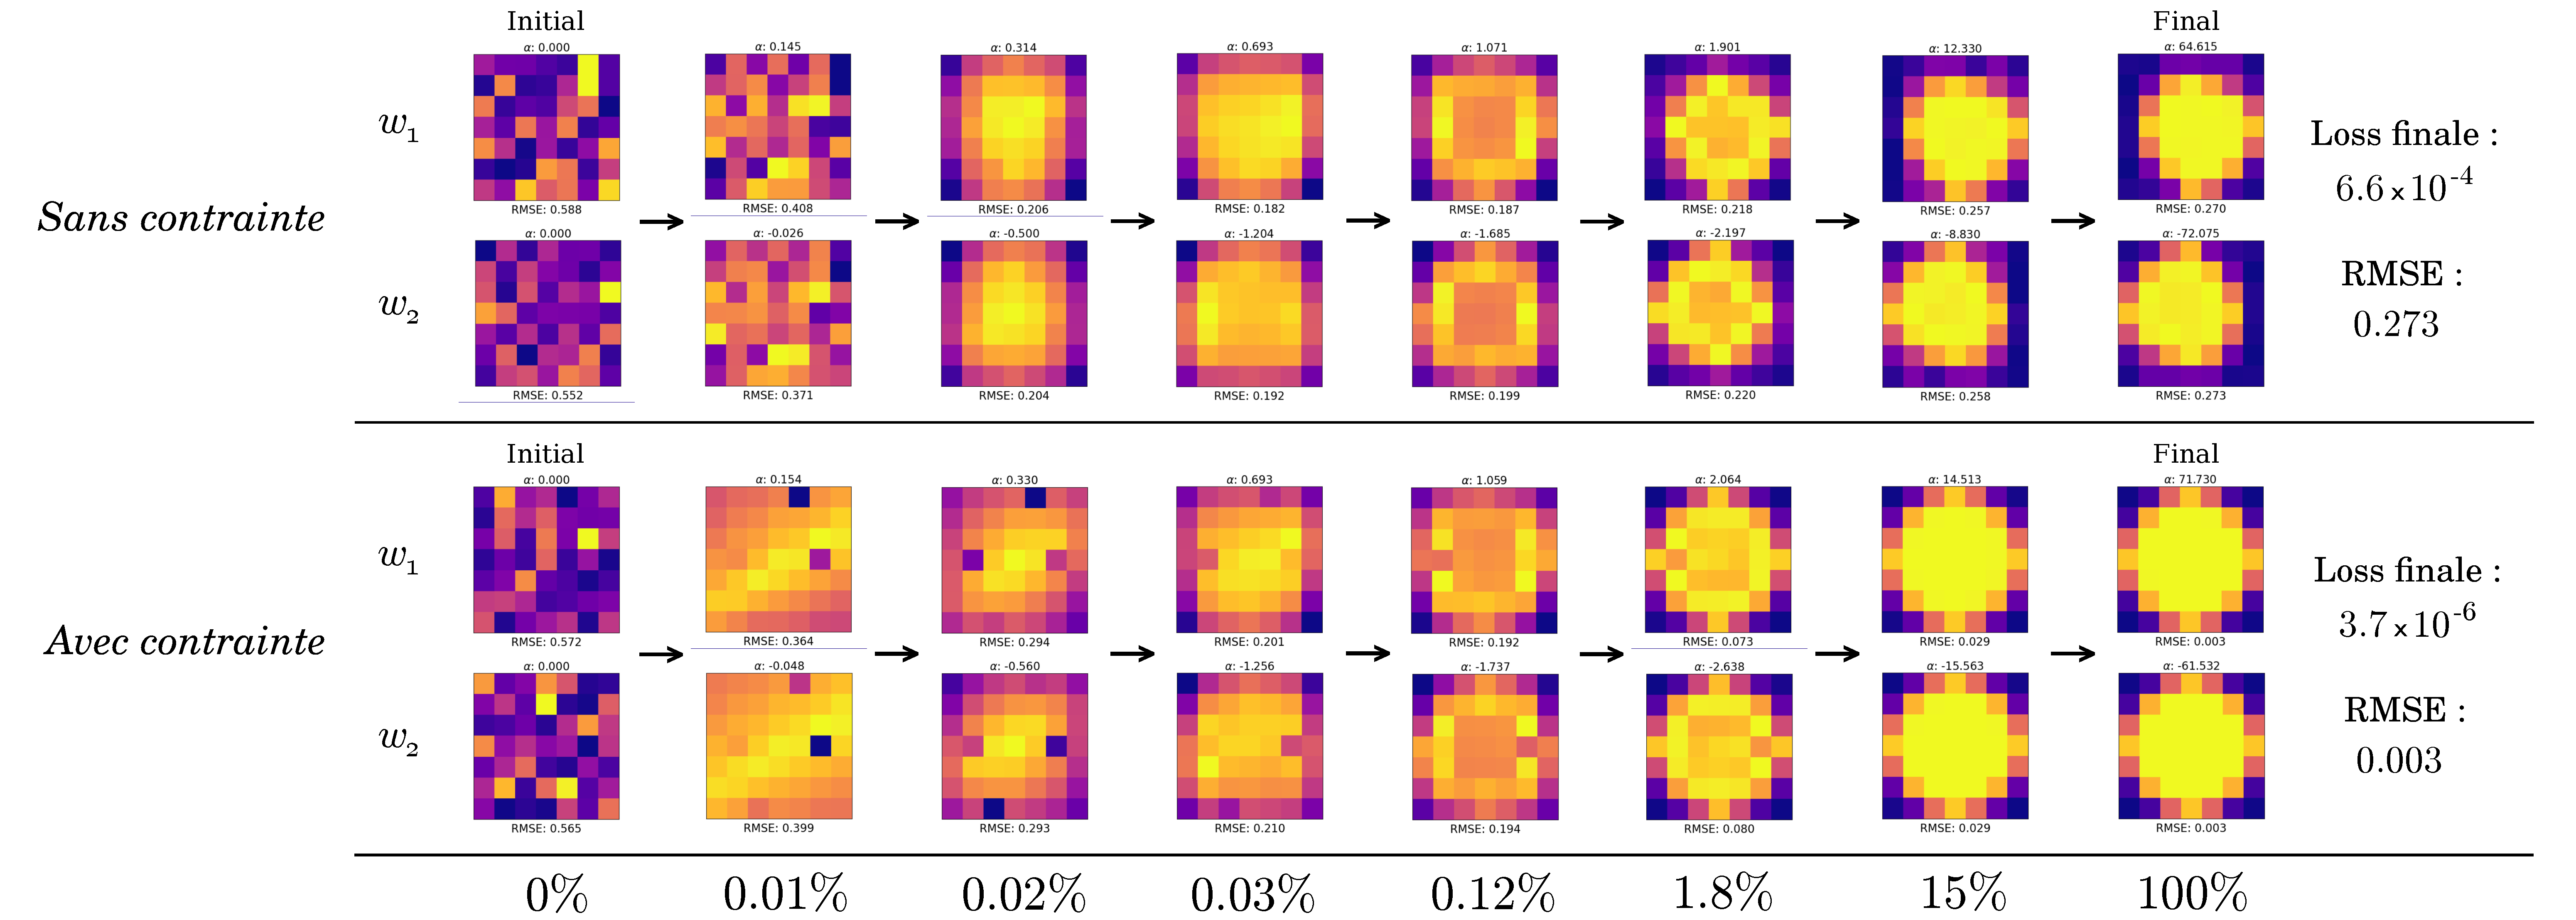
\includegraphics[width=1.00\linewidth]{parts/3-contributions/C-contraintes_geometriques/figures/k_center.pdf}
    \vspace{-4.0mm}
    \caption{ \centering Évolution de la forme du noyau des deux couches du réseau et de sa \textit{RMSE} en fonction de la progression de l'entraînement (en \% avant l'état final), pour le \textit{disk3} et la fermeture sur la banque FashionMNIST, avec et sans la contrainte $C_\text{center}$.}
    \label{fig:c_center}
  \end{center}
\end{figure}

\vspace{-0.2mm}
\noindent On voit sur la figure \ref{fig:c_center} que, sur cette expérience par exemple, avec la structure \textit{disk3} pour la fermeture et la banque FashionMNIST, cette métrique est très efficace pour avoir à la fois une \textit{RMSE} faible (la forme du noyau $w$ ressemble bien à la structure cible) et à la fois une \textit{loss} faible (le réseau a bien convergé).
Cependant, cette contrainte ne peut typiquement pas être appliquée dans le cas de fonctions structurantes cibles pour lesquelles le centre de masse est éloigné du centre du support, ou est inconnu. Comme expliqué dans les motivations, on ne pourra ainsi appliquer cette contrainte que dans des contextes particuliers où les informations nécessaires sont connues. \\


%%%%%%%%%%%%%%%%%%%%%%%%%%%%%%%%%%%%%%%%%%%%%%%%%%%%%%%%%%%%%%%%%%%%%%%%%%%%%%%%%%%%%%%%%%%%%%%%%%%%%%%%%%%%%%
%%%%%%%%%%%%%%%%%%%%%%%%%%%%%%%%%%%%%%%%%%%%% 2e contrainte %%%%%%%%%%%%%%%%%%%%%%%%%%%%%%%%%%%%%%%%%%%%%%%%%%
%%%%%%%%%%%%%%%%%%%%%%%%%%%%%%%%%%%%%%%%%%%%%%%%%%%%%%%%%%%%%%%%%%%%%%%%%%%%%%%%%%%%%%%%%%%%%%%%%%%%%%%%%%%%%%

\newpage

\noindent \textbf{b. Erreur sur la dispersion}\\

La deuxième métrique de contrainte géométrique sur les noyaux $w$ est l'erreur sur la dispersion, notée $C_\text{disp}$. Alors que l'erreur sur le centre de masse peut être associée à une moyenne (biais), l'erreur sur la dispersion peut être, quant à elle, associée à une variance. Soit $p_c \in \mathbb{R}^2$ le point de << concentration >> visé (en pratique, $p_c = p_w$), et soit $\zeta > 0$ (par défaut, $\zeta = 2$). L'erreur $C_\text{disp}$ sur la dispersion de $w$ par rapport à $p_c$ est définie par :

\vspace{-1.4mm}
\begin{equation}
    C_\text{disp}(w, p_c)_\zeta = \frac{ 1 }{ \sup_{p \in W} \left \| p - p_c \right \| ^\zeta } \frac{ 1 }{ \sum_{p \in W} w(p) } \sum_{p \in W} \left \| p - p_c \right \| ^\zeta w(p)
    \label{erreur_disp}
\end{equation}

\vspace{4.6mm}
%\noindent En pratique, on prendra : $p_c = p_w$ . \\

%\vspace{-2.0mm}
\noindent Prenons par exemple l'expérience avec \textit{disk2} pour la fermeture sur MNIST. La figure ci-après montre l'évolution de la convergence des deux noyaux du réseau, avec des checkpoints à différents stades durant l'entraînement, sans et avec cette contrainte $C_\text{disp}$ dans la \textit{loss} (avec $\lambda = 0.01$). Dans les deux cas, le réseau possède encore le partage de poids doux décrit précédemment. On obtient les mêmes résultats sur 6 runs. \\

%%% A chaque fois, faire deux comparaisons (schéma de l'évolution du filtre sur plusieurs périodes) : l'une sans la contrainte (prendre un truc qui converge mal), l'autre avec (prendre un truc qui converge bien) !

%figure
\vspace{0.4mm}
\begin{figure}[htp]
  \begin{center}
    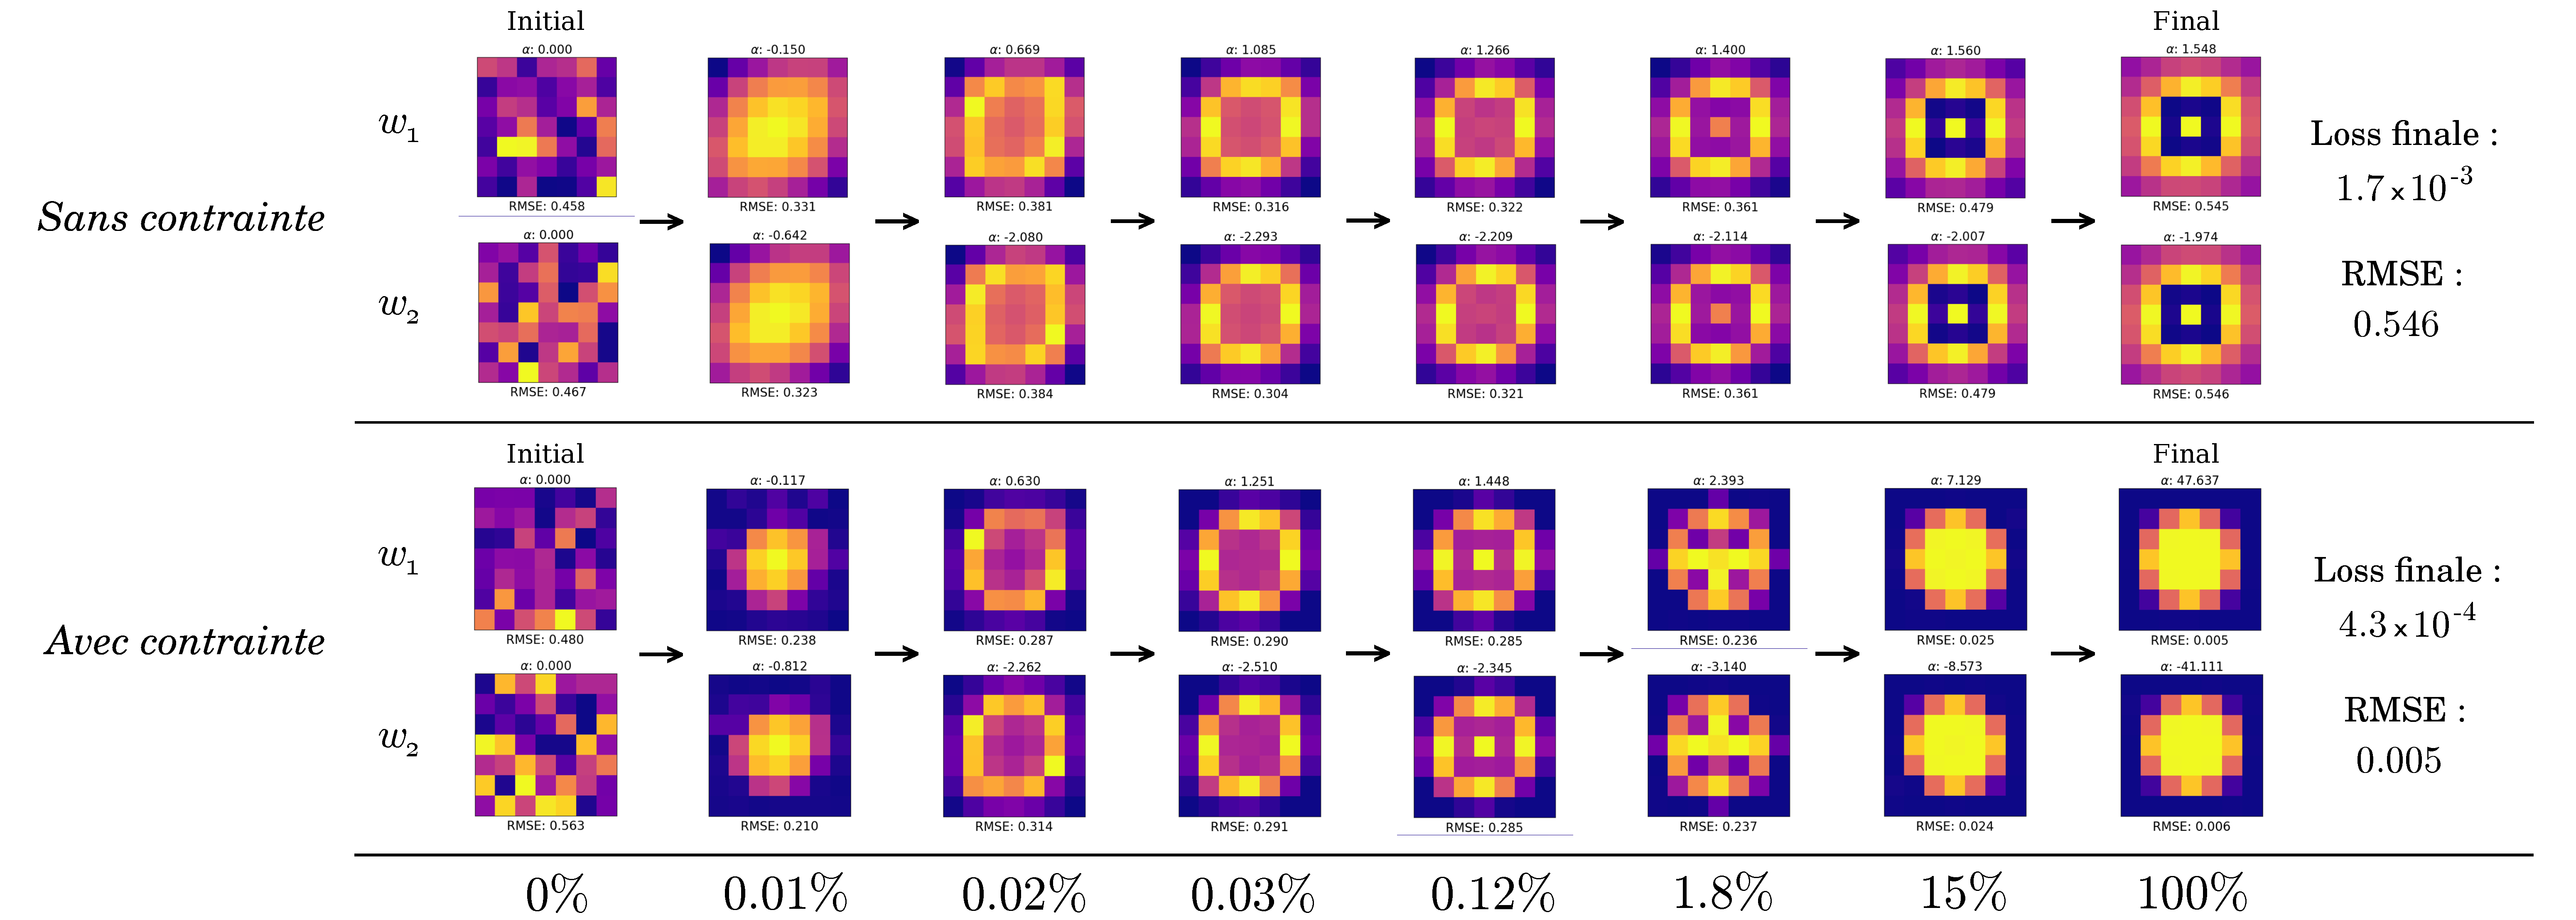
\includegraphics[width=1.00\linewidth]{parts/3-contributions/C-contraintes_geometriques/figures/k_disp.pdf}
    \vspace{-4.0mm}
    \caption{ \centering Évolution de la forme du noyau des deux couches du réseau et de sa \textit{RMSE} en fonction de la progression de l'entraînement (en \% avant l'état final), pour le \textit{disk2} et la fermeture sur la banque MNIST, avec et sans la contrainte $C_\text{disp}$.}
    \label{fig:c_disp}
  \end{center}
\end{figure}

\vspace{-1.6mm}
\noindent On voit sur la figure \ref{fig:c_disp} que, sur cette expérience par exemple, avec la structure \textit{disk2} pour la fermeture et la banque MNIST, cette métrique est très efficace pour avoir à la fois une \textit{RMSE} faible (la forme du noyau $w$ ressemble bien à la structure cible) et à la fois une \textit{loss} faible (le réseau a bien convergé).
Cependant encore, cette contrainte ne peut pas être appliquée dans le cas de fonctions structurantes cibles pour lesquelles les poids sont dispersés sur le support, ou dont la configuration est inconnue.


%%%%%%%%%%%%%%%%%%%%%%%%%%%%%%%%%%%%%%%%%%%%%%%%%%%%%%%%%%%%%%%%%%%%%%%%%%%%%%%%%%%%%%%%%%%%%%%%%%%%%%%%%%%%%%
%%%%%%%%%%%%%%%%%%%%%%%%%%%%%%%%%%%%%%%%%%%%% 3e contrainte %%%%%%%%%%%%%%%%%%%%%%%%%%%%%%%%%%%%%%%%%%%%%%%%%%
%%%%%%%%%%%%%%%%%%%%%%%%%%%%%%%%%%%%%%%%%%%%%%%%%%%%%%%%%%%%%%%%%%%%%%%%%%%%%%%%%%%%%%%%%%%%%%%%%%%%%%%%%%%%%%

\newpage

\noindent \textbf{c. Erreur sur la symétrie}\\

La troisième métrique de contrainte géométrique sur les noyaux $w$ des réseaux morphologiques est l'erreur sur la symétrie, notée $C_\text{sym}$. Soit $p_c \in \mathbb{R}^2$ le centre de symétrie visé (en pratique, $p_c = p_w$), et soit $\zeta > 0$ (par défaut, $\zeta = 2$). L'erreur $C_\text{sym}$ sur la symétrie centrale de $w$ par rapport au point $p_c$ est définie par :

\vspace{2.0mm}
\begin{equation}
    C_\text{sym}(w, p_c)_\zeta = 
    \frac{ 
    \sum_{p \in W} 
    \begin{cases}
        \hspace{1.4mm} \left | \hspace{0.7mm} w(p) - w( 2 p_c - p ) \hspace{0.7mm} \right | ^\zeta & \mbox{si} \hspace{3mm} 2 p_c - p \in W \\
        \hspace{1.4mm} \left ( w(p) - \inf_{q \in W} \{ w(q) \} \right ) ^\zeta & \mbox{sinon}
    \end{cases}
    }
    { |W| \left ( \sup_{p \in W} \{ w(p) \} - \inf_{p \in W} \{ w(p) \} \right ) ^\zeta }
    \label{erreur_sym}
\end{equation}

\vspace{4.5mm}
\noindent Prenons par exemple l'expérience avec \textit{diamond3} pour la fermeture sur la banque FashionMNIST. La figure ci-après montre l'évolution de la convergence des deux noyaux du réseau, avec des checkpoints à différents stades durant l'entraînement, sans et avec cette contrainte $C_\text{sym}$ dans la \textit{loss} (avec $\lambda = 0.01$). Dans les deux cas, le réseau possède toujours un partage de poids doux. On obtient les mêmes résultats sur 6 runs. \\

%%% A chaque fois, faire deux comparaisons (schéma de l'évolution du filtre sur plusieurs périodes) : l'une sans la contrainte (prendre un truc qui converge mal), l'autre avec (prendre un truc qui converge bien) !

%figure
\vspace{-0.2mm}
\begin{figure}[htp]
  \begin{center}
    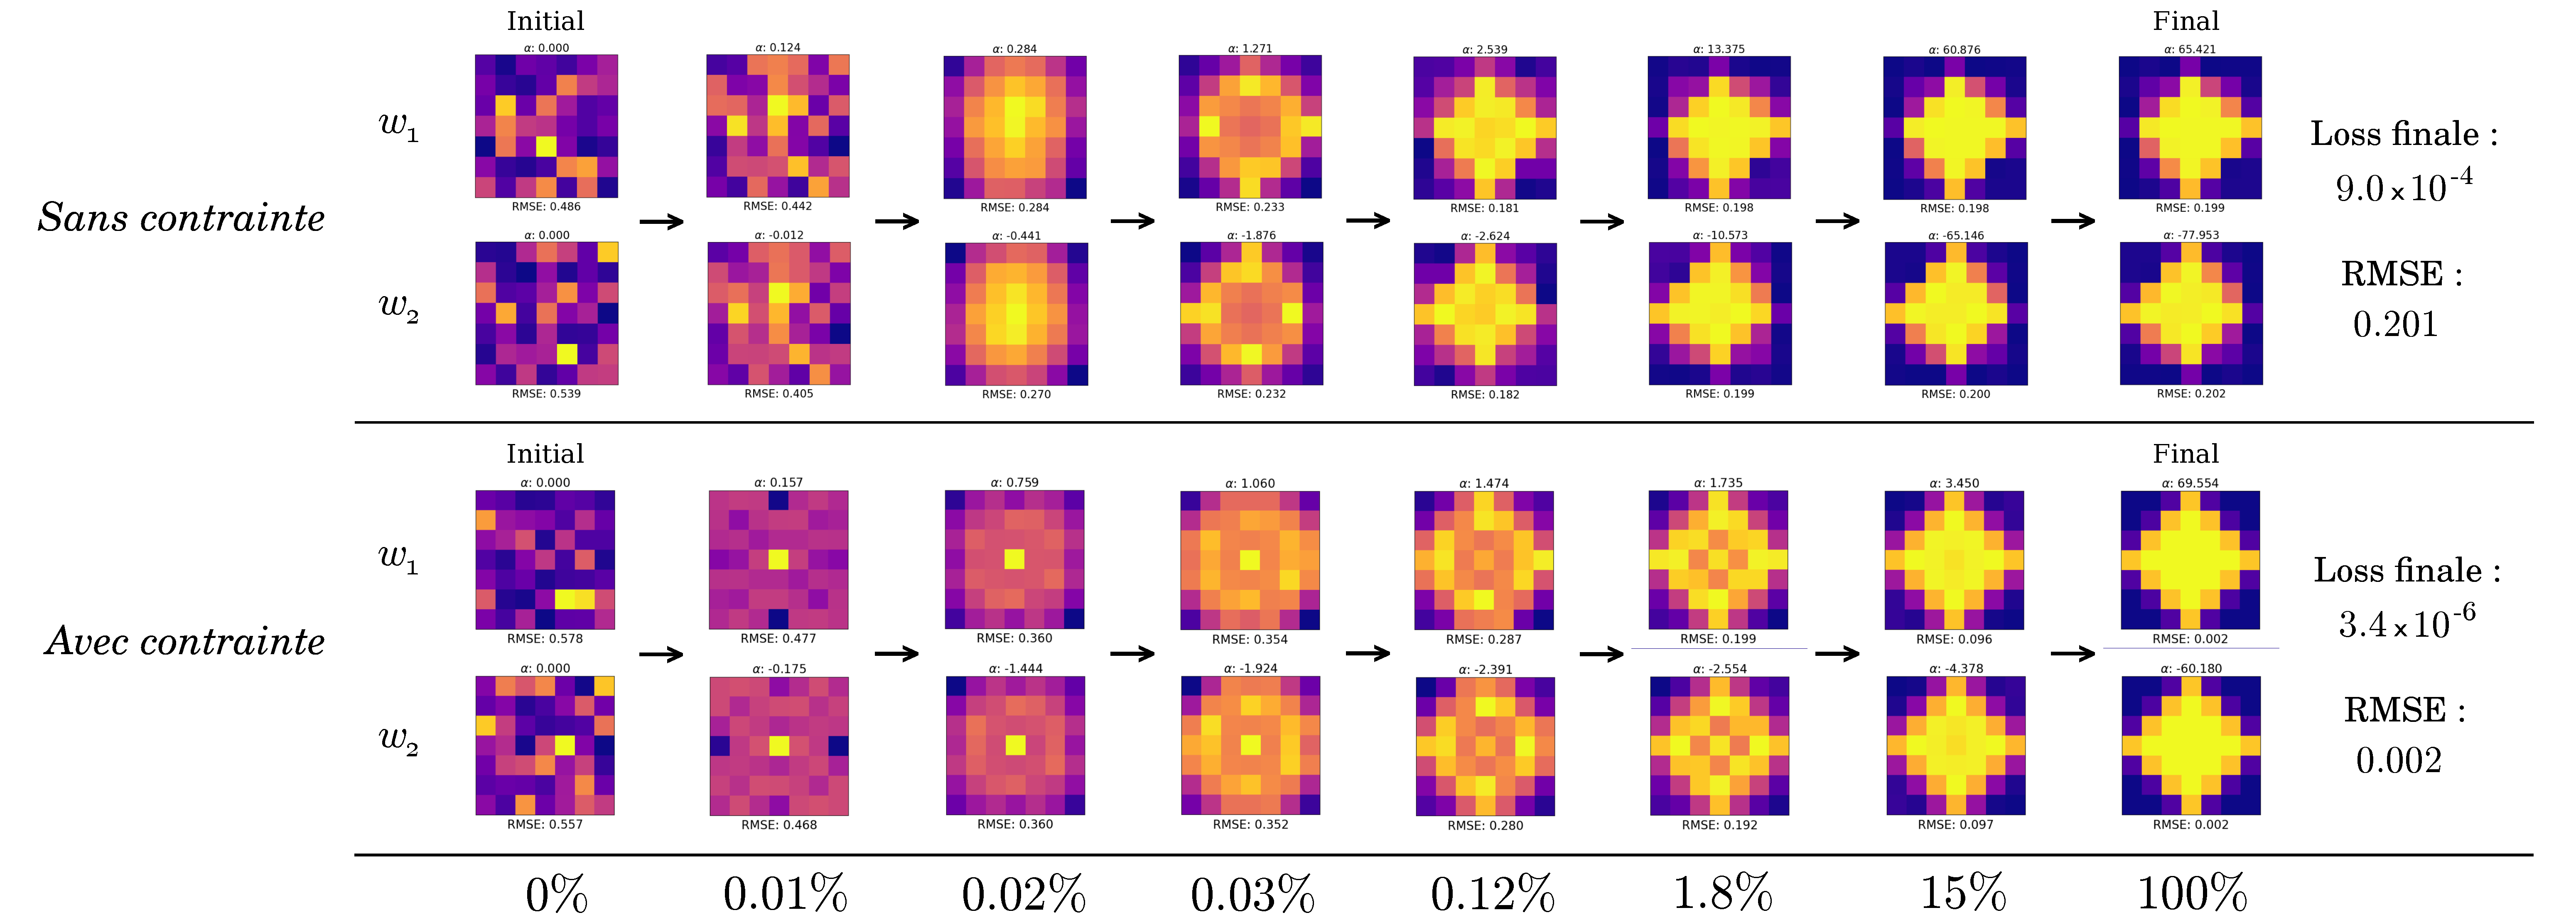
\includegraphics[width=1.00\linewidth]{parts/3-contributions/C-contraintes_geometriques/figures/k_sym.pdf}
    \vspace{-4.0mm}
    \caption{ \centering Évolution de la forme du noyau des deux couches du réseau et de sa \textit{RMSE} en fonction de la progression de l'entraînement (en \% avant l'état final), pour le \textit{diamond3} et la fermeture sur la banque FashionMNIST, avec et sans la contrainte $C_\text{sym}$.}
    \label{fig:c_sym}
  \end{center}
\end{figure}

\vspace{-2.4mm}
\noindent On voit sur la figure \ref{fig:c_sym} que, sur cette expérience par exemple, avec la structure cible symétrique \textit{diamond3} pour la fermeture et la banque FashionMNIST, cette métrique est efficace pour avoir à la fois une \textit{RMSE} faible (le noyau $w$ est proche de la structure cible) et à la fois une \textit{loss} faible (le réseau a bien convergé).
Encore une fois, cette contrainte ne peut cependant pas être appliquée dans le cas de fonctions structurantes cibles non symétriques (centralement), ou si le centre de symétrie est inconnu.


%%%%%%%%%%%%%%%%%%%%%%%%%%%%%%%%%%%%%%%%%%%%%%%%%%%%%%%%%%%%%%%%%%%%%%%%%%%%%%%%%%%%%%%%%%%%%%%%%%%%%%%%%%%%%%
%%%%%%%%%%%%%%%%%%%%%%%%%%%%%%%%%%%%%%%%%%%%% 4e contrainte %%%%%%%%%%%%%%%%%%%%%%%%%%%%%%%%%%%%%%%%%%%%%%%%%%
%%%%%%%%%%%%%%%%%%%%%%%%%%%%%%%%%%%%%%%%%%%%%%%%%%%%%%%%%%%%%%%%%%%%%%%%%%%%%%%%%%%%%%%%%%%%%%%%%%%%%%%%%%%%%%

\newpage

\noindent \textbf{d. Erreur sur la binarité}\\

La quatrième métrique de contrainte géométrique sur les noyaux $w$ des réseaux morphologiques est l'erreur sur la binarité, notée $C_\text{binary}$. Elle permet de faire converger les poids de $w$ vers deux bornes pré-définies, une inférieure $b_\text{inf} \in \mathbb{R}$ et une supérieure $b_\text{sup} \in \mathbb{R}$, avec $b_\text{sup} > b_\text{inf}$. En pratique, $b_\text{inf} = \inf_{p \in W} \{ w(p) \}$ et $b_\text{sup} = \sup_{p \in W} \{ w(p) \}$. Pour $\zeta > 0$ (par défaut, $\zeta = 2$), l'erreur $C_\text{binary}$ sur la binarité des poids de $w$ aux bornes $b_\text{inf}$ et $b_\text{sup}$ est définie par :

\vspace{-0.4mm}
\begin{equation}
    C_\text{binary}(w, (b_\text{inf}, b_\text{sup}))_\zeta = 
    \frac{1}{ |W| } 
    \sum_{p \in W} 
    \left |
    1 - \left | \frac{ 2 w(p) - b_\text{sup} - b_\text{inf} }{ b_\text{sup} - b_\text{inf} } \right | ^\zeta
    \right | ^\zeta
    \label{erreur_binary}
\end{equation}

\vspace{4.5mm}
\noindent Prenons par exemple l'expérience avec \textit{brand} pour la fermeture sur la banque MNIST. La figure ci-après montre l'évolution de la convergence des deux noyaux du réseau, avec des checkpoints à différents stades durant l'entraînement, sans et avec cette contrainte $C_\text{binary}$ dans la \textit{loss} (avec $\lambda = 0.0001$). Dans les deux cas, le réseau possède toujours un partage de poids doux. On obtient les mêmes résultats sur 6 runs. \\

%%% A chaque fois, faire deux comparaisons (schéma de l'évolution du filtre sur plusieurs périodes) : l'une sans la contrainte (prendre un truc qui converge mal), l'autre avec (prendre un truc qui converge bien) !

%figure
\vspace{-0.4mm}
\begin{figure}[htp]
  \begin{center}
    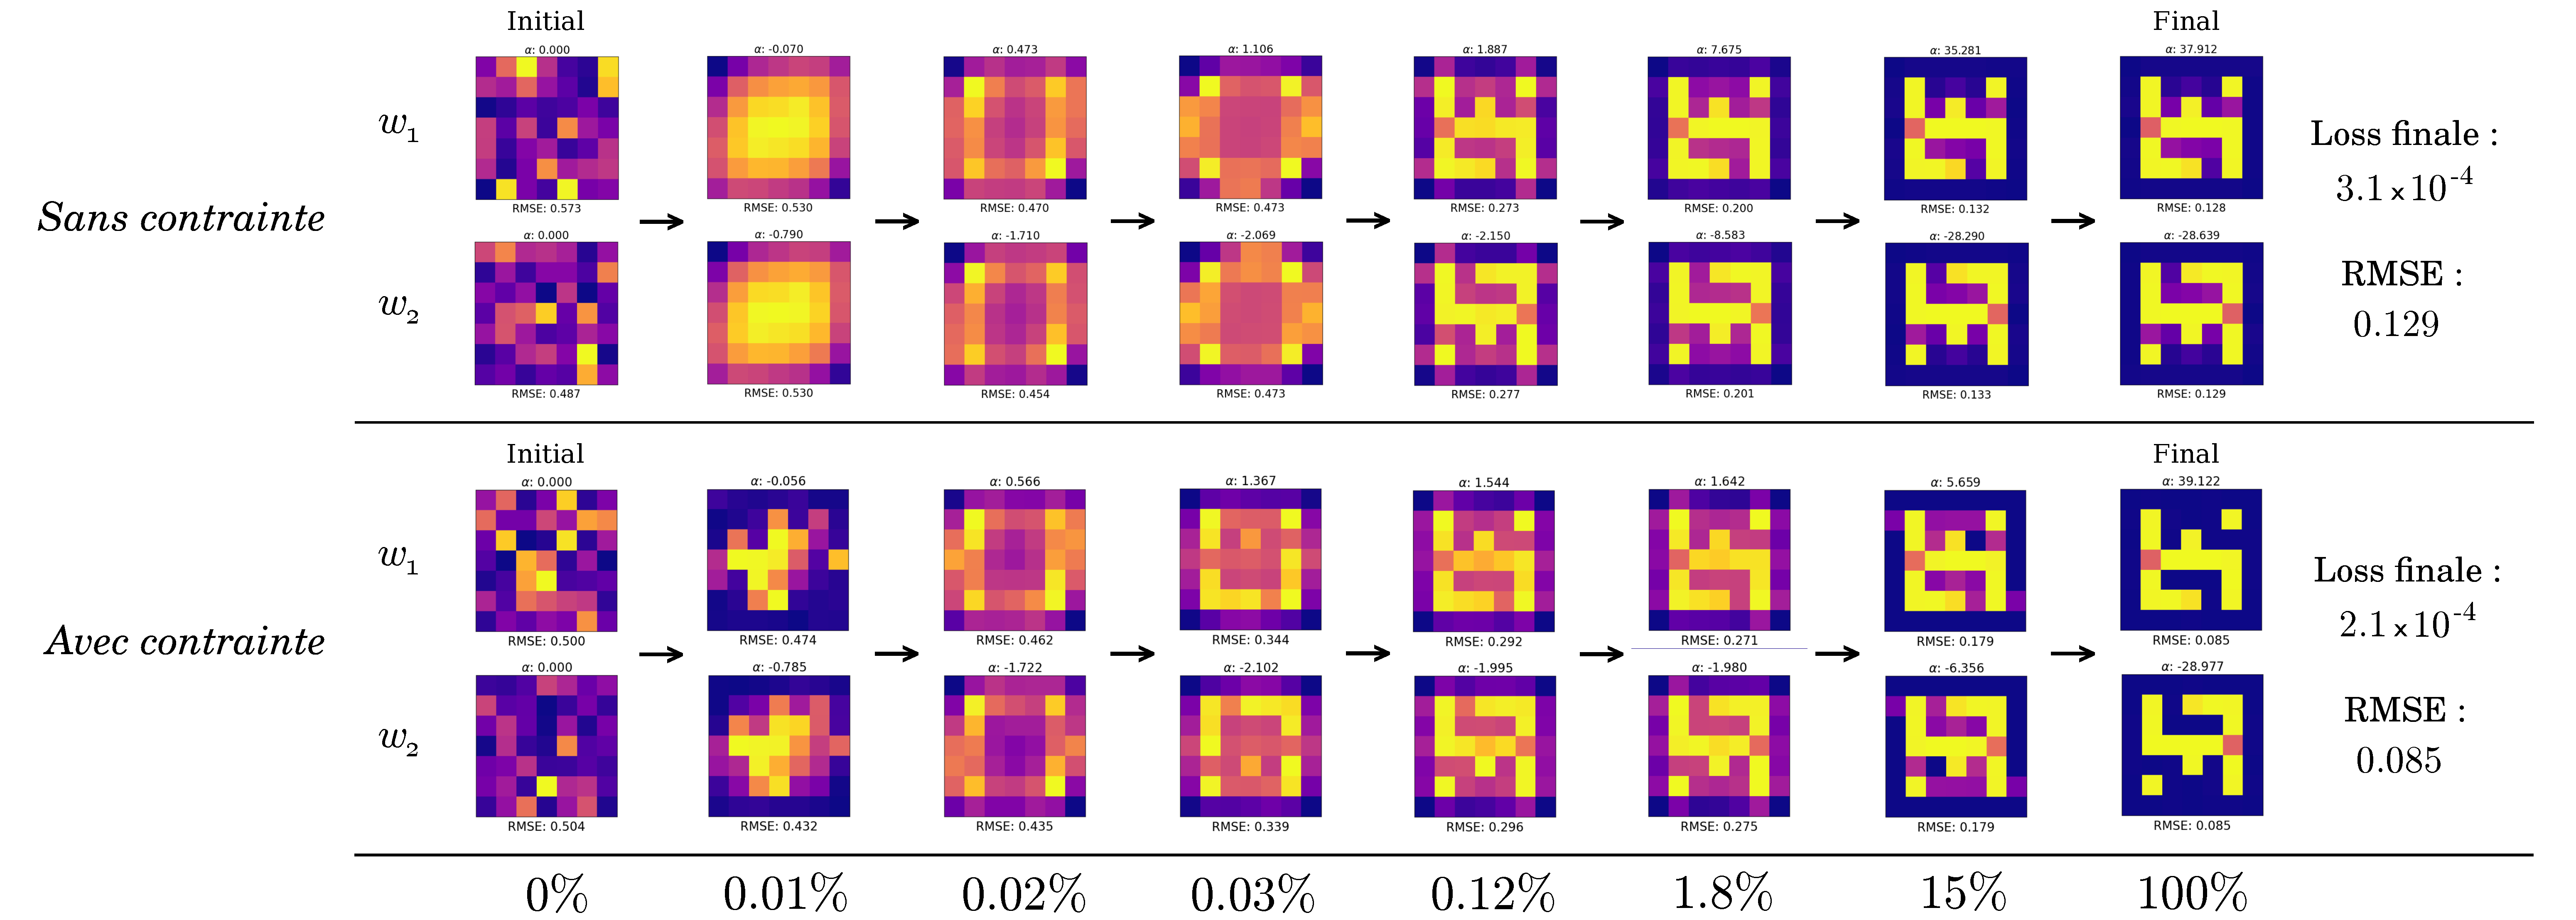
\includegraphics[width=1.00\linewidth]{parts/3-contributions/C-contraintes_geometriques/figures/k_binary.pdf}
    \vspace{-4.0mm}
    \caption{ \centering Évolution de la forme du noyau des deux couches du réseau et de sa \textit{RMSE} en fonction de la progression de l'entraînement (en \% avant l'état final), pour le \textit{brand} et la fermeture sur la banque MNIST, avec et sans la contrainte $C_\text{binary}$.}
    \label{fig:c_binary}
  \end{center}
\end{figure}

\vspace{-2.6mm}
\noindent On voit sur la figure \ref{fig:c_binary} que, sur cette expérience par exemple, avec la structure cible \textit{brand} pour la fermeture et la banque MNIST, cette métrique permet effectivement de mieux binariser les poids du noyau, et permet également une légère amélioration de la convergence du réseau, aussi bien sur la \textit{loss} que sur la \textit{RMSE}. Note : les images affichées sont les symétriques des noyaux $w$.
Précisons également que cette contrainte n'a pas de pertinence dans le cas de fonctions structurantes cibles non binaires.


%%%%%%%%%%%%%%%%%%%%%%%%%%%%%%%%%%%%%%%%%%%%%%%%%%%%%%%%%%%%%%%%%%%%%%%%%%%%%%%%%%%%%%%%%%%%%%%%%%%%%%%%%%%%%%
%%%%%%%%%%%%%%%%%%%%%%%%%%%%%%%%%%%%%%%%%%%%% 4e contrainte %%%%%%%%%%%%%%%%%%%%%%%%%%%%%%%%%%%%%%%%%%%%%%%%%%
%%%%%%%%%%%%%%%%%%%%%%%%%%%%%%%%%%%%%%%%%%%%%%%%%%%%%%%%%%%%%%%%%%%%%%%%%%%%%%%%%%%%%%%%%%%%%%%%%%%%%%%%%%%%%%

\newpage

\noindent \textbf{e. Erreur sur la norme}\\

La dernière métrique de contrainte géométrique sur les noyaux $w$ est l'erreur sur leur norme, notée $C_\text{norm}$. Elle permet à la norme du noyau de converger vers une valeur cible prédéfinie $l_c \in \mathbb{R}_+$. Par défaut, $l_c = 0$. L'erreur $C_\text{norm}$ sur la norme $n$, avec $n > 0$ (par défaut, $n = 1$), du noyau $w$ est définie, avec $\zeta > 0$ (par défaut, $\zeta = 2$), par :

%\vspace{-0.0mm}
\begin{equation}
    C_\text{norm}(w, l_c)_{n,\zeta} = 
    \frac
    { \left | 
    \left ( \sum_{p \in W} \left | w(p) \right | ^n \right ) ^{1/n} - l_c
    \right | ^\zeta }
    { |W| ^ {\zeta/n} \left ( \sup_{p \in W} \{ w(p) \} - \inf_{p \in W} \{ w(p) \} \right ) ^\zeta } 
    \label{erreur_norm}
\end{equation}

\vspace{4.5mm}
Par défaut, $n = 1$, car la norme \textit{1} est le meilleur approximateur convexe de la norme $0$ (on s'intéresse à la norme $0$ pour calculer la taille de l'<< objet >> du support). \\
%, i.e. le nombre de pixels de valeur strictement supérieure à 0). \\

\vspace{-2.6mm}
\noindent Prenons l'expérience avec \textit{complex} pour la fermeture sur la banque FashionMNIST. La figure ci-après montre l'évolution de la convergence des deux noyaux du réseau durant l'entraînement, sans et avec la contrainte $C_\text{norm}$ dans la \textit{loss} (avec $\lambda = 0.001$). Le réseau a toujours un partage de poids doux. On obtient ces résultats sur 6 runs. \\

%%% A chaque fois, faire deux comparaisons (schéma de l'évolution du filtre sur plusieurs périodes) : l'une sans la contrainte (prendre un truc qui converge mal), l'autre avec (prendre un truc qui converge bien) !

%figure
\vspace{-0.8mm}
\begin{figure}[htp]
  \begin{center}
    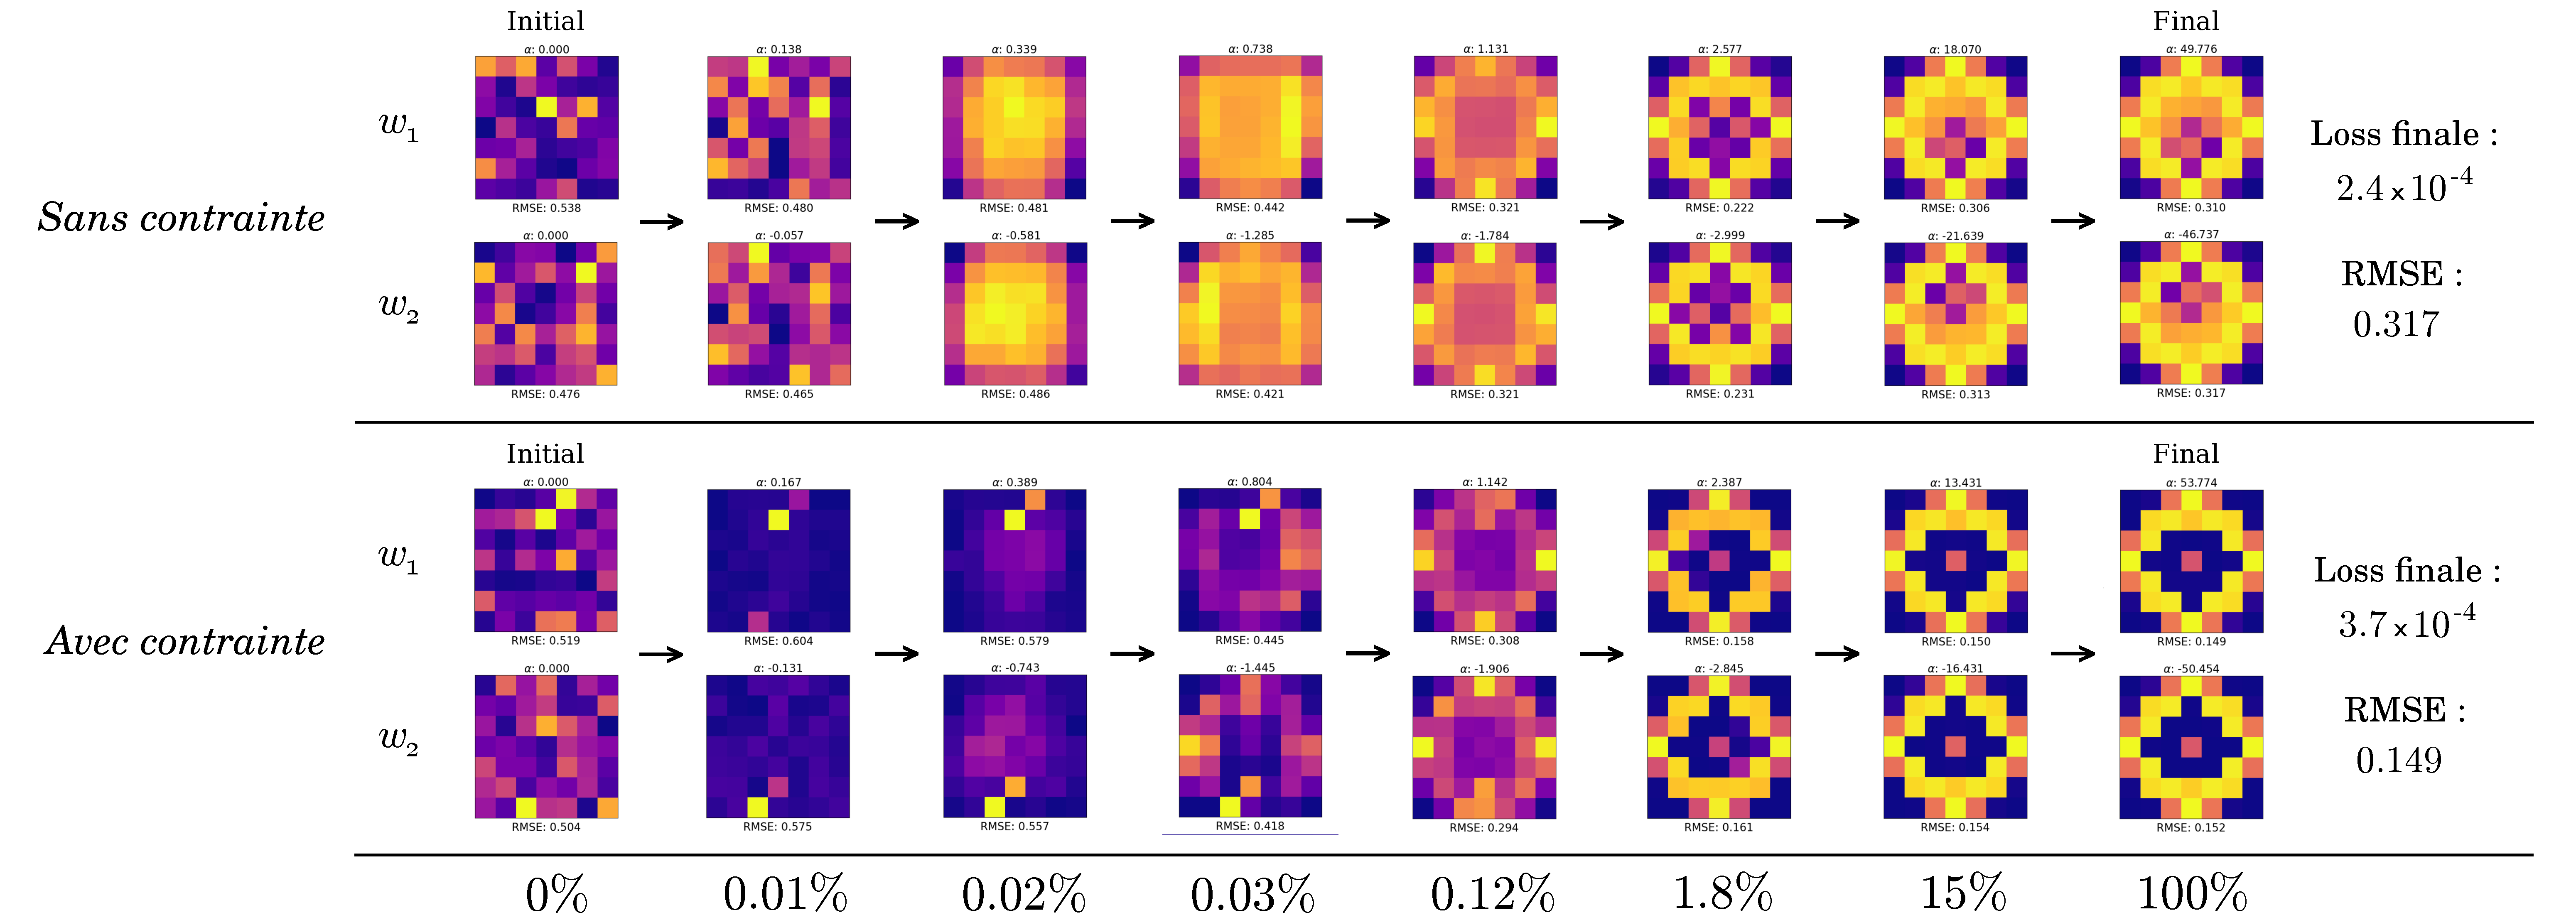
\includegraphics[width=1.00\linewidth]{parts/3-contributions/C-contraintes_geometriques/figures/k_norm.pdf}
    \vspace{-4.0mm}
    \caption{ \centering Évolution de la forme du noyau des deux couches du réseau et de sa \textit{RMSE} en fonction de la progression de l'entraînement (en \% avant l'état final), pour le \textit{complex} et la fermeture sur la banque FashionMNIST, avec et sans la contrainte $C_\text{norm}$.}
    \label{fig:c_norm}
  \end{center}
\end{figure}

\vspace{-3.0mm}
\noindent Cette contrainte permet de réduire le nombre de pixels nuisibles et d'artéfacts sur $w$ si l'hyperparamètre $\lambda$ est bien ajusté dans la \textit{loss}. Les résultats de la figure \ref{fig:c_norm} avec cette contrainte (où $l_c = 0$ et $\lambda = 0.001$) sont meilleurs en terme de \textit{RMSE}, mais un peu moins bons en terme de \textit{loss} par rapport à ceux sans $C_\text{norm}$.
Cette contrainte étant utilisée en particulier pour minimiser le nombre de pixels apparents dans $w$, elle peut donc être utilisée dans tout contexte si on veut avoir un objet minimal dans $w$ sur $W$.


\newpage

\noindent \textbf{Remarque pour l'ensemble des contraintes sur $w$ :} \\

\vspace{-1.0mm}
\noindent Dans les cas pratiques, on utilisera, pour ces cinq métriques de contraintes étudiées, le noyau $w$ \textit{normalisé}, écrit $\mathfrak{N}(w)$ (formule \ref{normalized}). Cela permet en particulier de distinguer l'<< objet >> (dont les valeurs sur $\mathfrak{N}(w)$ sont près de $1$) du << fond >> (dont les valeurs sur $\mathfrak{N}(w)$ sont près de $0$) sur le support $W$. De plus, si on est avec les réseaux $\mathcal{S}$MorphNet (classique, sans tangente hyperbolique Tanh) ou $\mathcal{L}$MorphNet, et si le paramètre $\alpha/p$ associé au noyau $w$ est négatif, alors on prend la négation $-w$ au lieu de $w$.
